% filepath: /Users/momen_mac/Desktop/flutter_application/report/chapters/04_system_design.tex
\chapter{System Design}
\label{ch:system_design}

This chapter presents the comprehensive system design and architecture of LiveSpot, a real-time location-based social networking application. The design documentation encompasses functional and non-functional requirements, architectural patterns, UML models, database design, security considerations, and deployment strategies that collectively deliver a robust platform for location-verified community reporting and social interaction.

%%%%%%%%%%%%%%%%%%%%%%%%%%%%%%%%%%%%%%%%%%%%%%%%%%%%%%%%%%%%%%%%%%%%%%%%%%%%%%%%%%%
\section{Requirements Analysis}
\label{sec:requirements_analysis}

\subsection{Functional Requirements}

The system must provide essential functionality for location-based community reporting and social networking based on user needs and business objectives.

\begin{table}[h!]
    \centering
    \caption{Core Functional Requirements}
    \label{tab:functional_requirements}
    \begin{tabular}{lll}     
        \toprule
        Requirement ID & Description & Priority \\
        \midrule
        FR001 & User account creation and secure authentication & Critical \\
        FR002 & Create location-verified posts with media content & Critical \\
        FR003 & View posts on interactive map interface & Critical \\
        FR004 & Browse and filter posts by category and location & Critical \\
        FR005 & Upvote/downvote posts and engage with content & High \\
        FR006 & User profile management and customization & High \\
        FR007 & Real-time notifications for relevant activities & High \\
        FR008 & Media file upload and storage capabilities & High \\
        FR009 & Search functionality for posts and users & Medium \\
        FR010 & Direct messaging between users & Medium \\
        FR011 & AI-powered assistant for recommendations and help & Medium \\
        FR012 & Content reporting and moderation tools & Medium \\
        FR013 & Social features (following users, saved posts) & Low \\
        FR014 & Admin tools for content management & Low \\
        FR015 & Multi-platform access (mobile and web) & Low \\
        \bottomrule
    \end{tabular}
\end{table}

\subsection{Non-Functional Requirements}

The system design addresses critical quality attributes based on actual LiveSpot implementation characteristics and performance targets.

\begin{table}[h!]
    \centering
    \caption{Non-Functional Requirements}
    \label{tab:nonfunctional_requirements}
    \begin{tabular}{lll}     
        \toprule
        Category & Requirement & Target Metric \\
        \midrule
        Performance & API response time & <2 seconds (Django REST) \\
        Performance & Map tile loading & <1 second (OSM direct) \\
        Performance & App startup time & <3 seconds (Flutter optimized) \\
        Performance & AI response time & <5 seconds (Gemini API) \\
        Scalability & Concurrent users & 1,000+ users (PostgreSQL) \\
        Scalability & Message storage & Real-time Firestore + Django \\
        Scalability & Database growth & Horizontal scaling ready \\
        Availability & OpenStreetMap uptime & 99.9\% (external dependency) \\
        Availability & Backend uptime & 99.5\% (Django server) \\
        Reliability & JWT token security & 15-minute access tokens \\
        Reliability & Data consistency & ACID compliance (PostgreSQL) \\
        Usability & Cross-platform UI & Consistent Flutter Material Design \\
        Usability & Offline capability & Map caching and local storage \\
        Security & Authentication & JWT + Google OAuth hybrid \\
        Security & Data encryption & HTTPS/TLS for all communications \\
        Cost Efficiency & External services & Free OSM + paid fallbacks \\
        \bottomrule
    \end{tabular}
\end{table}

%%%%%%%%%%%%%%%%%%%%%%%%%%%%%%%%%%%%%%%%%%%%%%%%%%%%%%%%%%%%%%%%%%%%%%%%%%%%%%%%%%%
\section{System Architecture Overview}
\label{sec:system_architecture}

LiveSpot implements a hybrid mobile-first architecture combining cross-platform mobile development with cloud-based backend services using a layered architectural pattern.

\begin{figure}[h!]
    \centering
    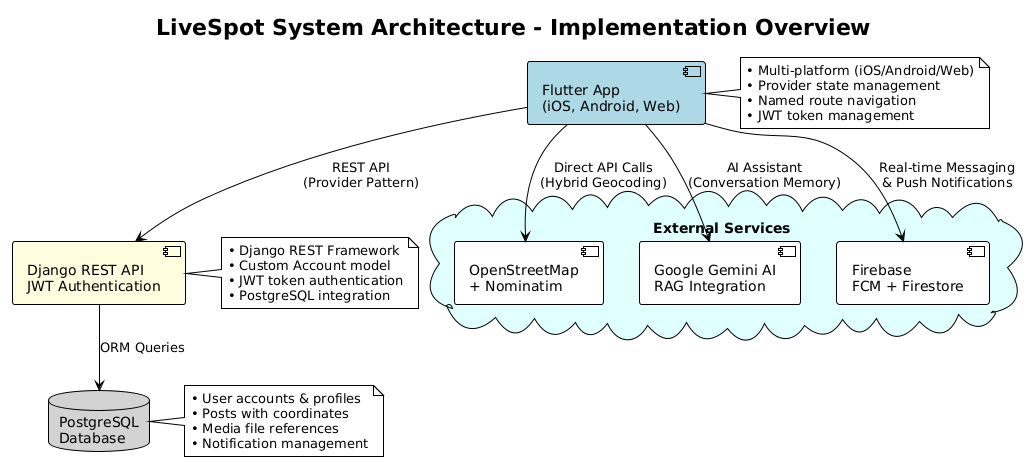
\includegraphics[width=0.9\textwidth]{figures/system_architecture}
    \caption{LiveSpot System Architecture Overview - Comprehensive view of the hybrid mobile-first architecture showing Flutter client, Django REST backend, PostgreSQL database, and external service integrations}
    \label{fig:system_architecture}
\end{figure}

Figure~\ref{fig:system_architecture} illustrates the complete system architecture encompassing all major components and their interactions. The architecture reflects the actual technology stack and service integrations implemented in the LiveSpot application, emphasizing the separation of concerns and scalable design patterns.

\subsection{Architectural Layers}

The architecture comprises three primary layers with clear separation of concerns:

\begin{itemize}
    \item \textbf{Presentation Layer:} Flutter cross-platform application with Provider state management and named routing
    \item \textbf{Business Logic Layer:} Django REST API backend with JWT authentication and service integrations
    \item \textbf{Data Layer:} PostgreSQL database with external service integrations (OSM, Gemini AI, Firebase)
\end{itemize}

\subsection{Architectural Patterns}

The system employs proven architectural patterns based on actual implementation:
\begin{itemize}
    \item \textbf{Provider Pattern:} Flutter state management with AccountProvider, PostsProvider, UserProfileProvider
    \item \textbf{REST API Architecture:} Django REST Framework with standardized endpoints and JWT authentication
    \item \textbf{Hybrid Service Integration:} OpenStreetMap primary with Google Geocoding fallback for cost optimization
    \item \textbf{RAG Integration:} Advanced AI assistant with contextual post retrieval and conversation memory
    \item \textbf{Multi-Platform Architecture:} Shared business logic across iOS, Android, and Web platforms
\end{itemize}

%%%%%%%%%%%%%%%%%%%%%%%%%%%%%%%%%%%%%%%%%%%%%%%%%%%%%%%%%%%%%%%%%%%%%%%%%%%%%%%%%%%
\section{Database Design}
\label{sec:database_design}

The database design follows PostgreSQL best practices with Django ORM integration, supporting the core functionality of location-based social networking with efficient relationships and data integrity.

\subsection{Entity Relationship Model}

The LiveSpot database architecture implements a comprehensive relational model designed to support real-time, location-based social networking functionality. The schema encompasses user management, content creation, social interactions, notification systems, and media storage with careful attention to performance optimization and data integrity.

\clearpage

\begin{figure}[p]
    \centering
    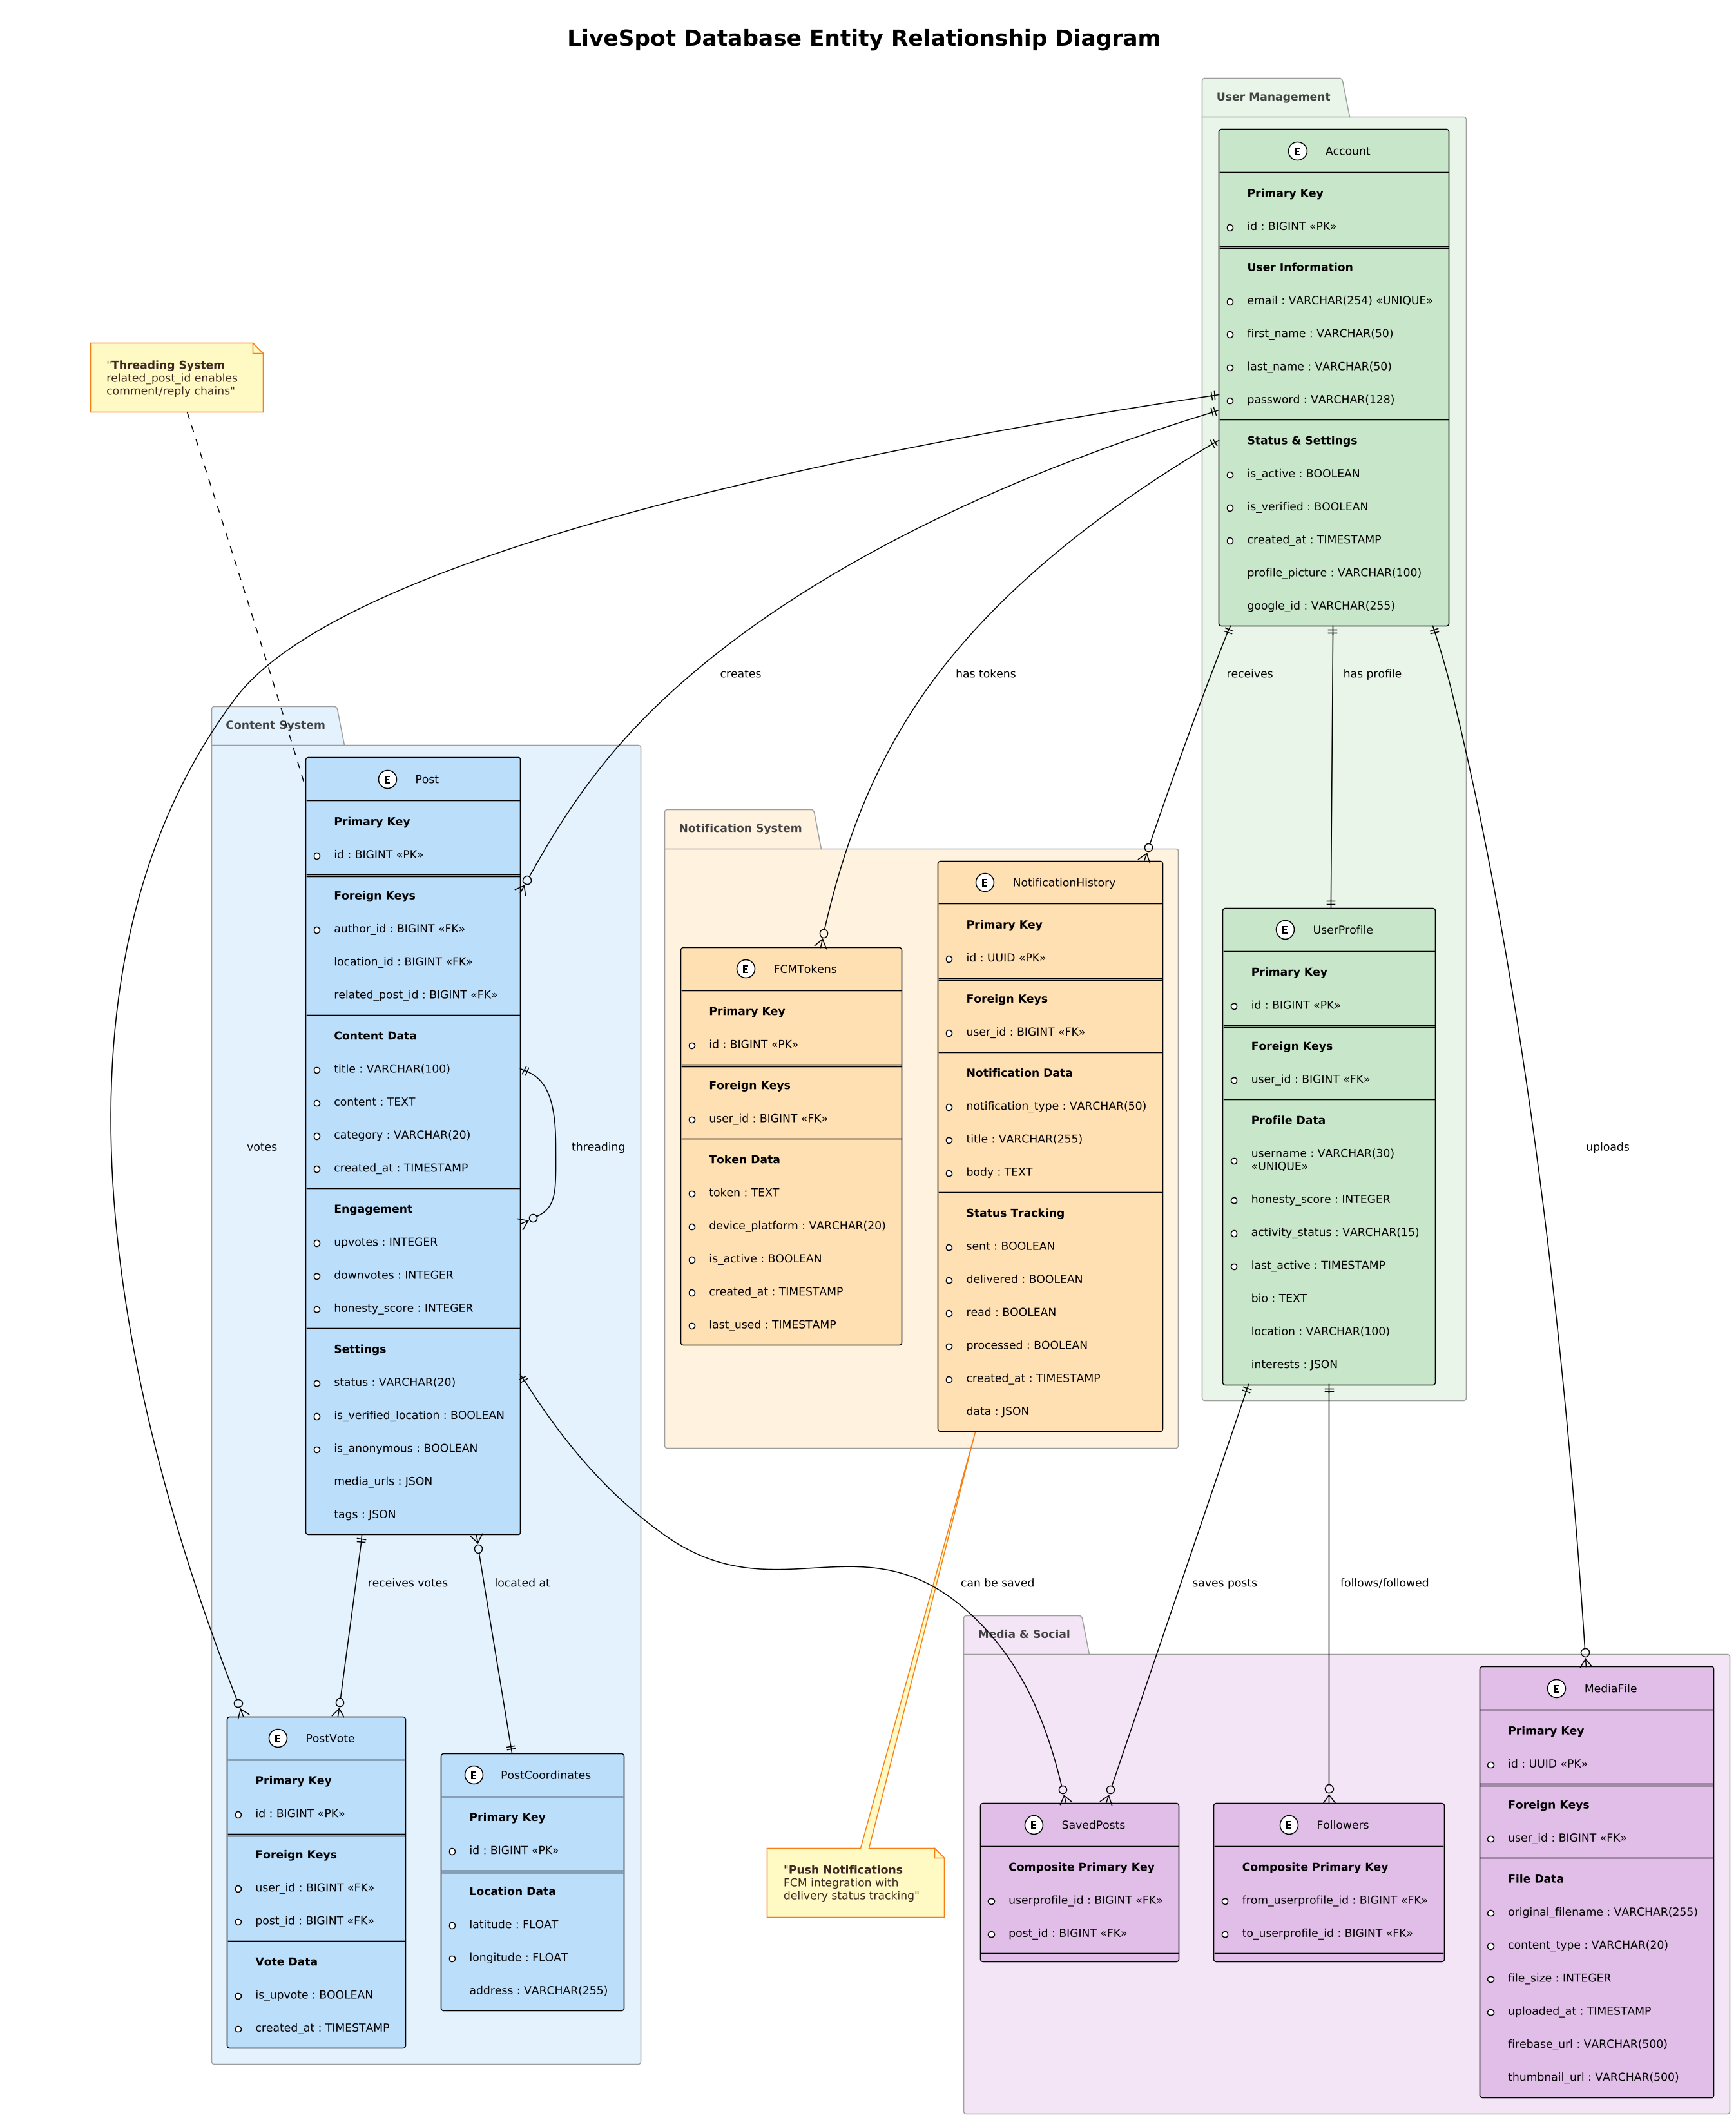
\includegraphics[width=\textwidth,height=0.9\textheight,keepaspectratio]{figures/database_erd}
    \caption{LiveSpot Database Entity Relationship Diagram - Complete schema showing all entities, relationships, and key attributes supporting location-verified social networking functionality}
    \label{fig:database_erd}
\end{figure}

\clearpage

The database schema illustrated in Figure~\ref{fig:database_erd} demonstrates the sophisticated relationship model underlying LiveSpot's functionality:

\textbf{Core User Management:}
\begin{itemize}
    \item \textbf{Account Entity:} Custom user model with authentication credentials, verification status, and account metadata
    \item \textbf{UserProfile Entity:} Extended user information including social features, activity tracking, and preference management
    \item \textbf{One-to-One Relationship:} Each account has exactly one profile, ensuring data consistency and optimal query performance
\end{itemize}

\textbf{Content and Location System:}
\begin{itemize}
    \item \textbf{Post Entity:} Central content model with threading support via \texttt{related\_post\_id} for comment-like functionality
    \item \textbf{PostCoordinates Entity:} Precise GPS location data with reverse-geocoded addresses for spatial queries
    \item \textbf{Threading Mechanism:} Self-referencing relationship enabling grouped discussions around specific events and locations
\end{itemize}

\textbf{Engagement and Social Features:}
\begin{itemize}
    \item \textbf{PostVote Entity:} User voting system with upvote/downvote functionality and duplicate prevention
    \item \textbf{SavedPosts Entity:} User bookmarking system with many-to-many relationship for content curation
    \item \textbf{Followers Entity:} Social networking capabilities enabling user-to-user following relationships
\end{itemize}

\textbf{Notification and Communication:}
\begin{itemize}
    \item \textbf{NotificationHistory Entity:} Comprehensive notification tracking with delivery status and metadata
    \item \textbf{FCMTokens Entity:} Push notification infrastructure supporting multiple devices per user
    \item \textbf{MediaFile Entity:} File storage management with Firebase integration for scalable media handling
\end{itemize}

\subsection{Firebase Integration}

Firebase services provide real-time messaging and push notification capabilities, complementing the PostgreSQL database for specific use cases that require instant delivery and offline synchronization.

% TODO: Add Firebase Data Model Diagram
% Figure~\ref{fig:firebase_schema} shows Firestore collections and document structure
\clearpage
%%%%%%%%%%%%%%%%%%%%%%%%%%%%%%%%%%%%%%%%%%%%%%%%%%%%%%%%%%%%%%%%%%%%%%%%%%%%%%%%%%%
\section{UML Sequence Diagrams}
\label{sec:sequence_diagrams}

The following sequence diagrams illustrate key user interaction flows and system behavior for critical LiveSpot functionality. Each diagram demonstrates the complete workflow for essential application features.

\subsection{User Authentication Flow}

The authentication system implements a secure JWT-based workflow with integrated FCM token registration for push notifications.

\begin{figure}[h!]
    \centering
    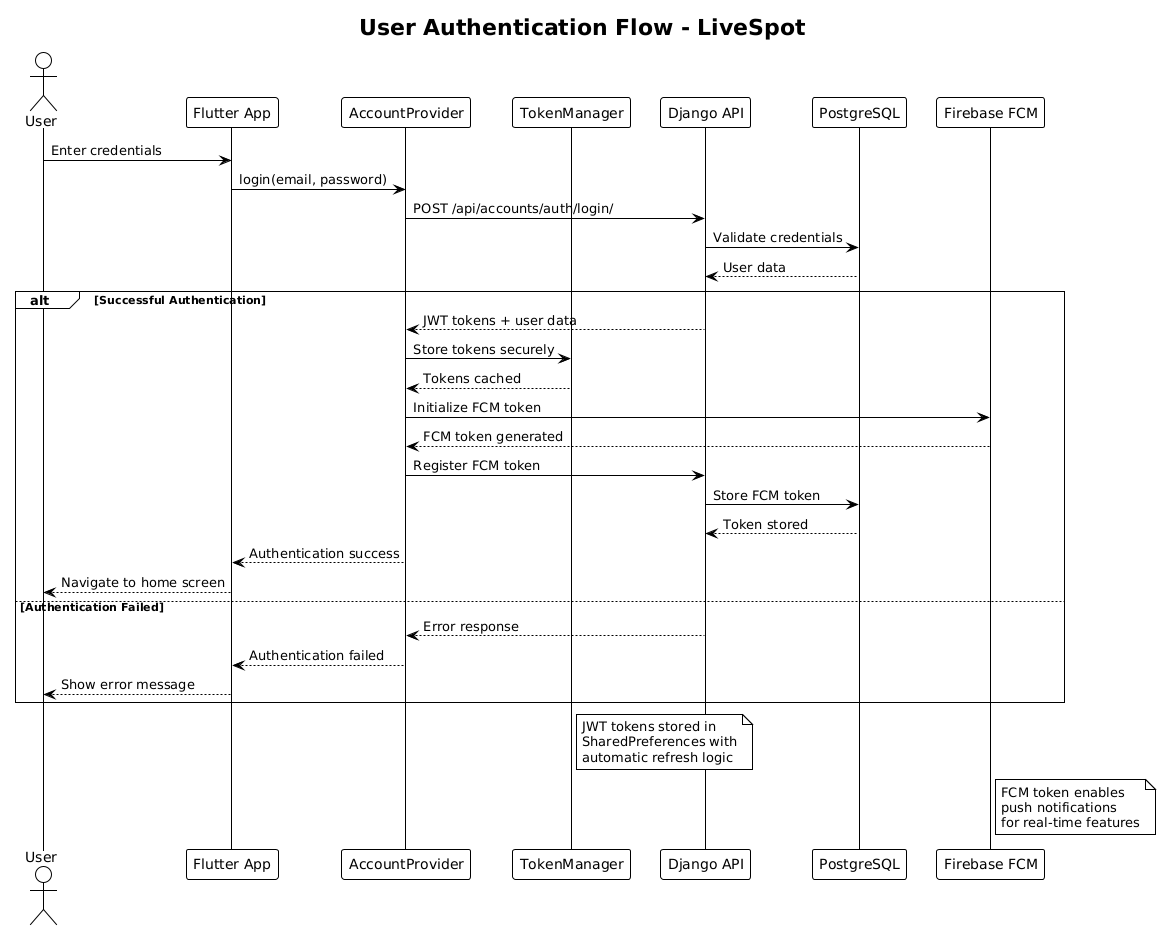
\includegraphics[width=0.95\textwidth]{figures/authentication_sequence}
    \caption{User Authentication Sequence Diagram - Complete JWT-based login flow showing credential validation, token generation, FCM registration, and session establishment}
    \label{fig:auth_sequence}
\end{figure}

Figure~\ref{fig:auth_sequence} demonstrates the comprehensive authentication workflow from initial user credential entry through successful JWT token storage and FCM token registration for push notifications. The sequence ensures secure user access while enabling real-time notification capabilities.
\clearpage
\subsection{Post Creation and Threading Flow}

The post creation system supports both standalone posts and threaded discussions with location verification and temporal constraints.

\begin{figure}[h!]
    \centering
    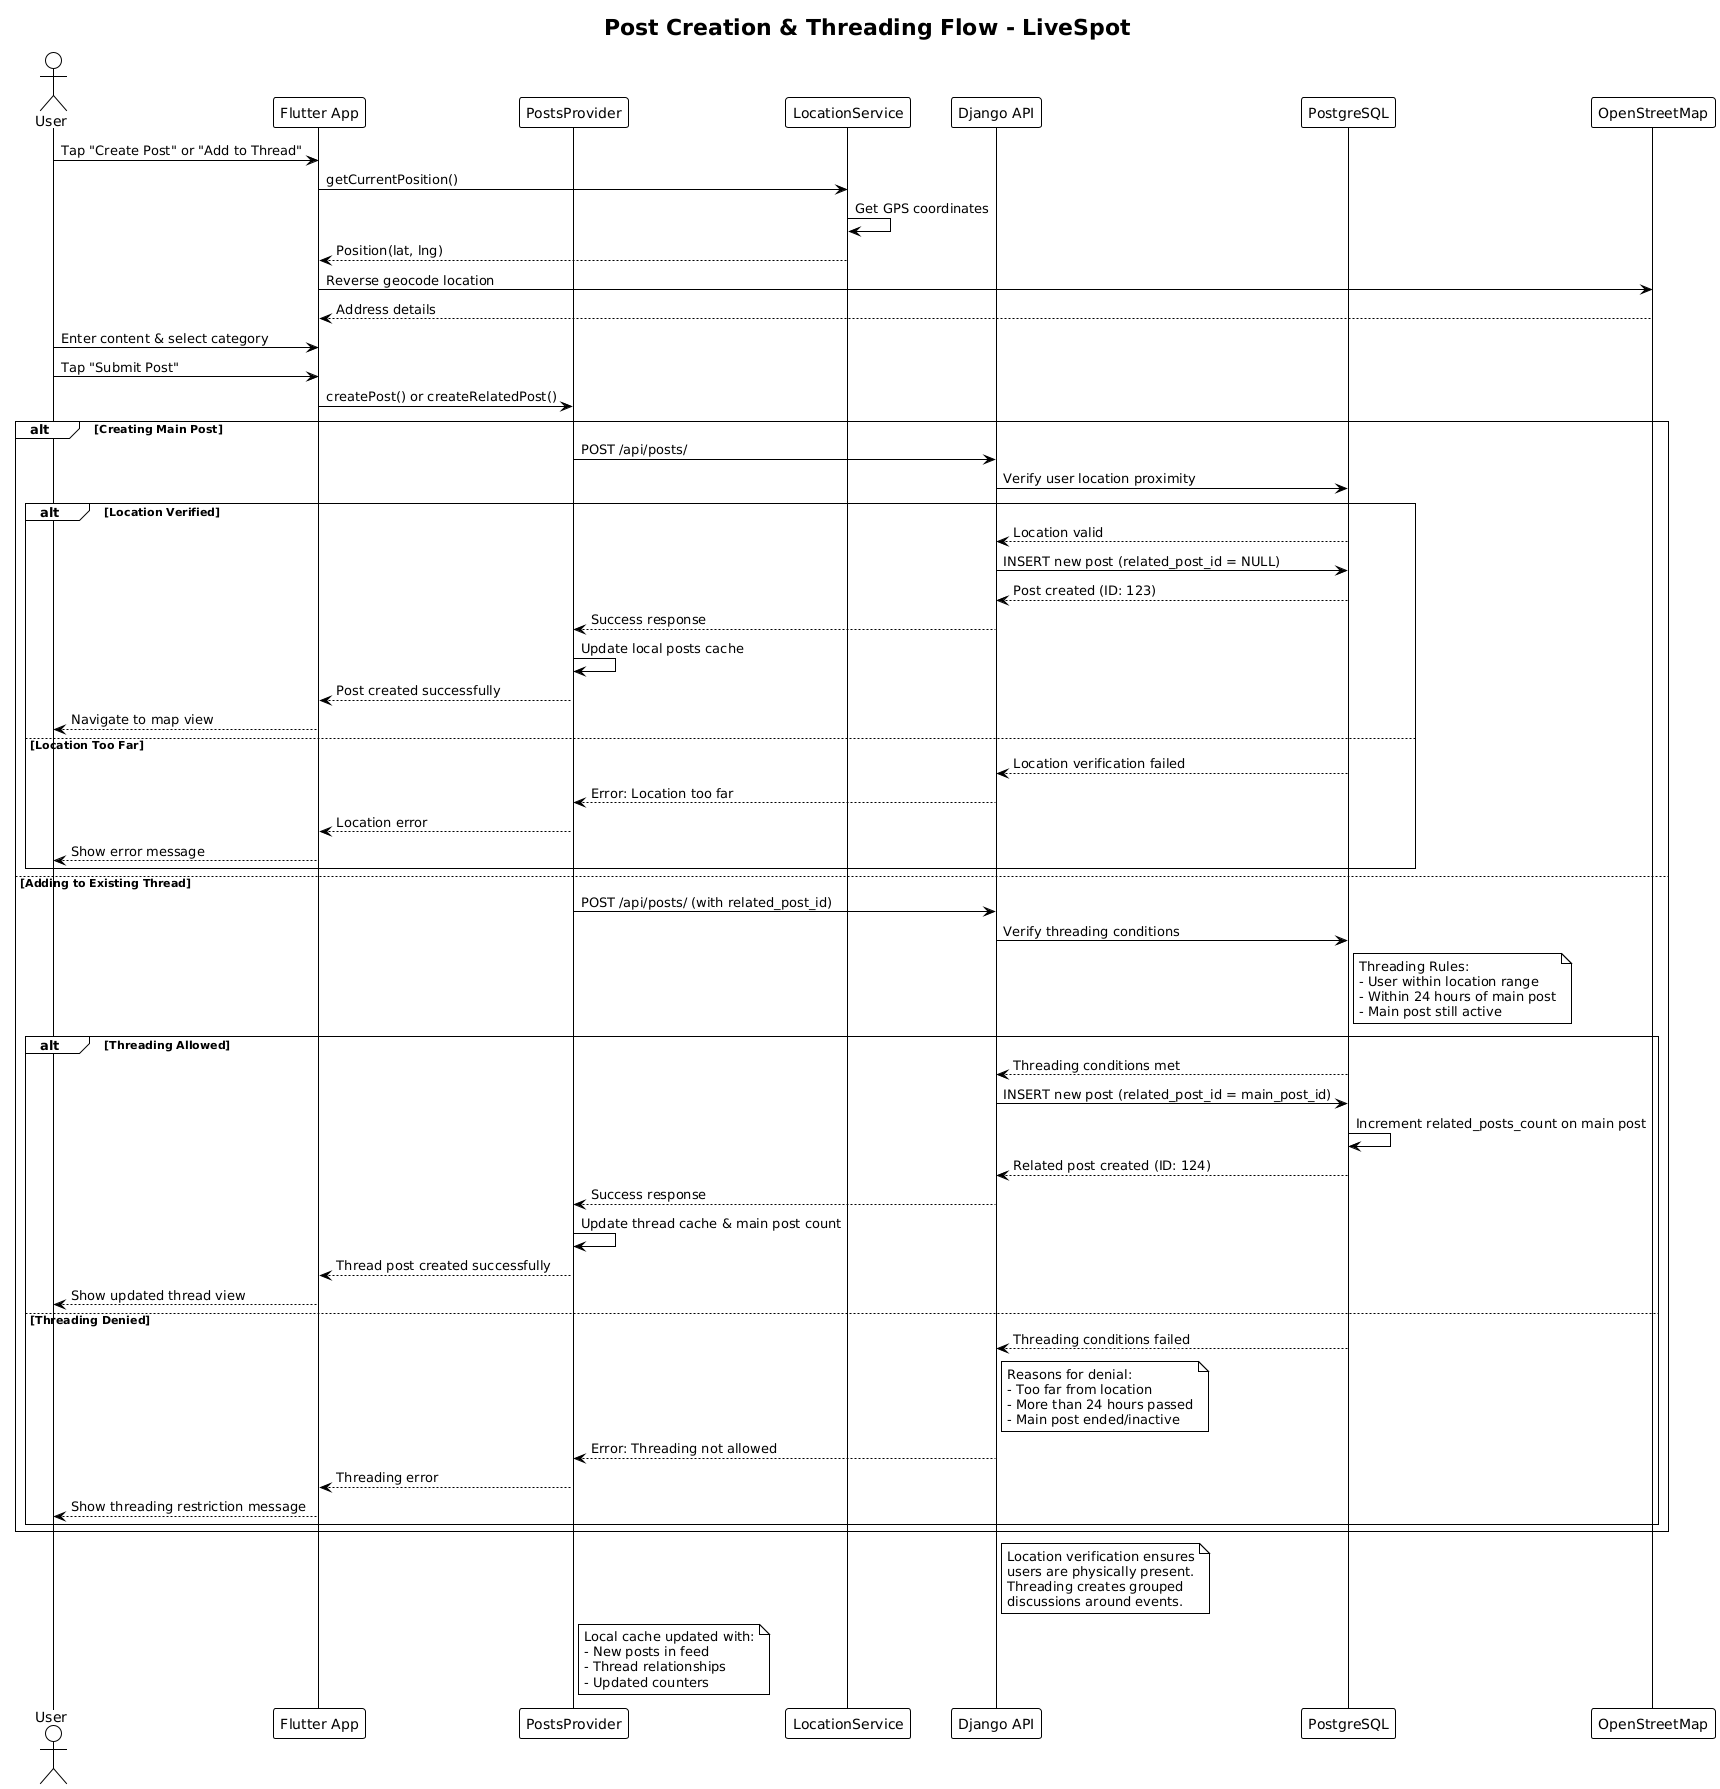
\includegraphics[width=\textwidth,height=0.75\textheight,keepaspectratio]{figures/post_creation_sequence}
    \caption{Post Creation and Threading Sequence Diagram}
    \label{fig:post_creation_sequence}
\end{figure}

Figure~\ref{fig:post_creation_sequence} illustrates the sophisticated post creation process encompassing location verification, reverse geocoding, threading decision logic, and database persistence. The diagram highlights the system's ability to create both main posts and related threaded posts with appropriate validation mechanisms.
\clearpage
\subsection{Real-time Messaging Flow}

The messaging architecture combines Firebase Firestore for real-time delivery with FCM for offline push notifications.

\begin{figure}[h!]
    \centering
    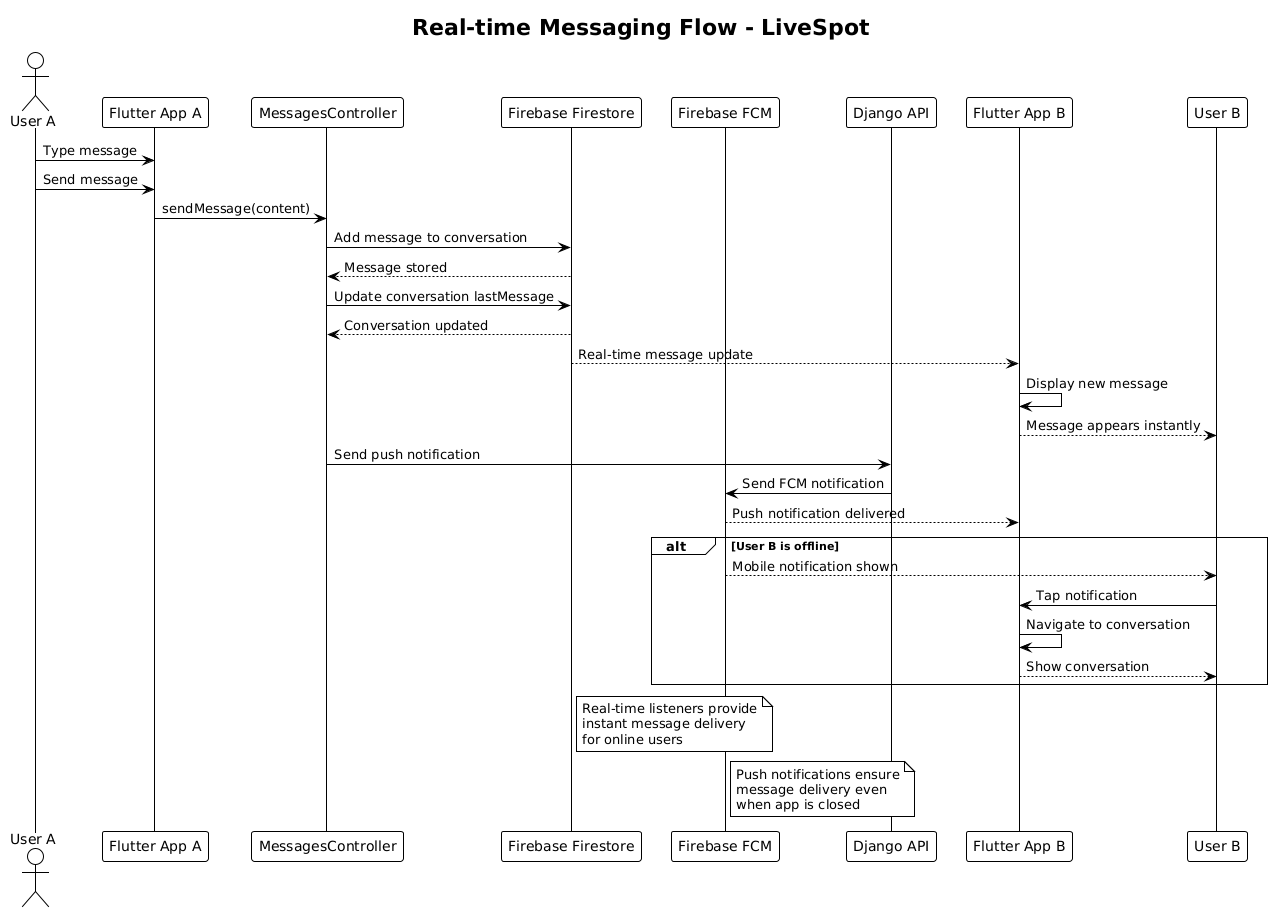
\includegraphics[width=0.95\textwidth]{figures/messaging_sequence}
    \caption{Real-time Messaging Sequence Diagram - Hybrid messaging architecture combining Firebase Firestore real-time synchronization with FCM push notifications for comprehensive communication coverage}
    \label{fig:messaging_sequence}
\end{figure}

Figure~\ref{fig:messaging_sequence} shows the hybrid messaging architecture that ensures reliable message delivery across different user states (online, offline, background). The system leverages Firebase Firestore for instant real-time synchronization and FCM for push notifications when users are not actively using the application.

%%%%%%%%%%%%%%%%%%%%%%%%%%%%%%%%%%%%%%%%%%%%%%%%%%%%%%%%%%%%%%%%%%%%%%%%%%%%%%%%%%%
\section{API Design and Integration}
\label{sec:api_design}

\subsection{RESTful API Architecture}

The LiveSpot API architecture implements a clean Django REST Framework backend with organized endpoint structure, JWT authentication, and external service integrations. The architecture supports cross-platform Flutter clients through standardized JSON communication patterns.

\begin{figure}[h!]
    \centering
    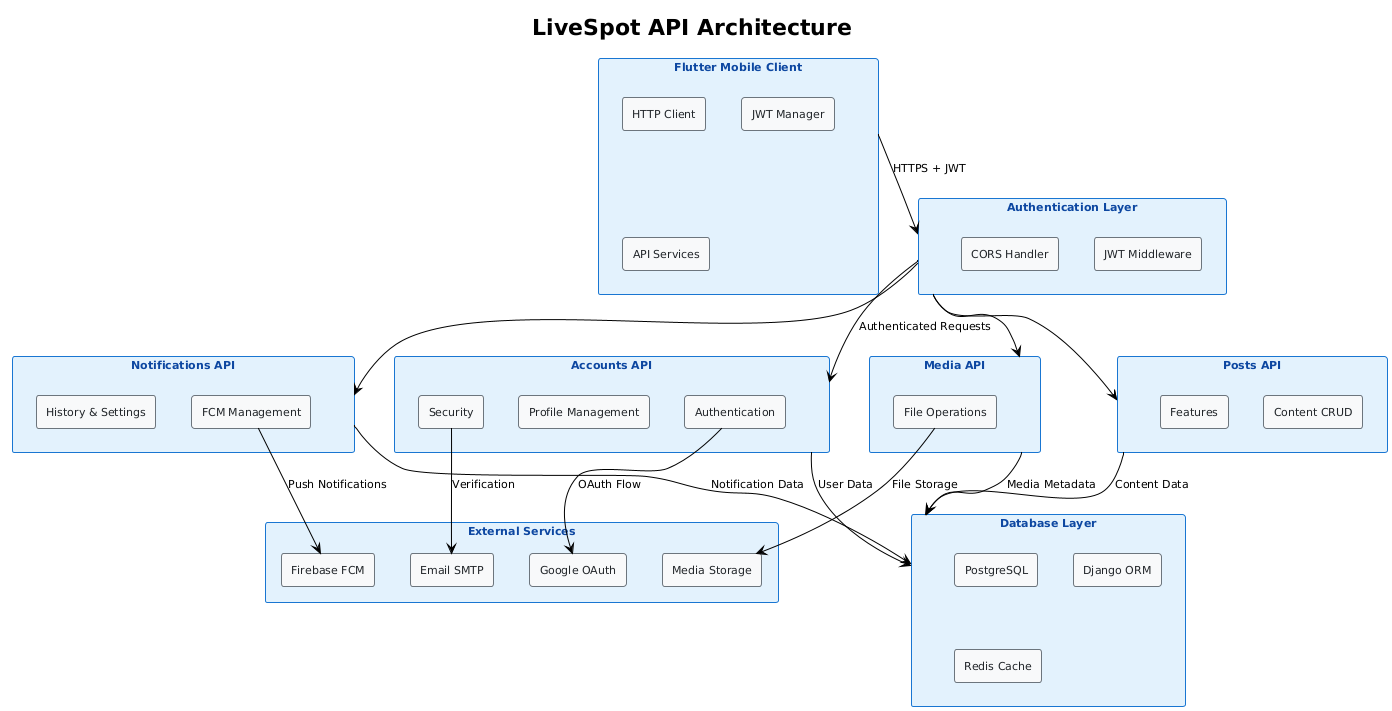
\includegraphics[width=0.8\textwidth]{figures/api_architecture}
    \caption{LiveSpot REST API Architecture - Vertical layout showing layered architecture from Flutter client through authentication middleware to organized API endpoints with external service integrations}
    \label{fig:api_architecture}
\end{figure}

Figure~\ref{fig:api_architecture} illustrates the vertical API architecture with clear separation between client, authentication, API endpoints, external services, and database layers. The design follows REST principles with organized endpoint grouping across four main domains: Accounts, Posts, Notifications, and Media APIs.

The architecture employs JWT middleware for secure authentication, CORS handling for cross-platform access, and seamless integration with external services including Firebase for notifications, Google OAuth for authentication, and cloud storage for media files. This layered approach ensures scalable, maintainable API design that supports the Flutter mobile application's requirements.

\subsection{External Service Integration}

Integration with third-party services expands functionality and improves user experience while maintaining cost-effectiveness and reliability through strategic service selection and hybrid approaches.

\begin{figure}[h!]
    \centering
    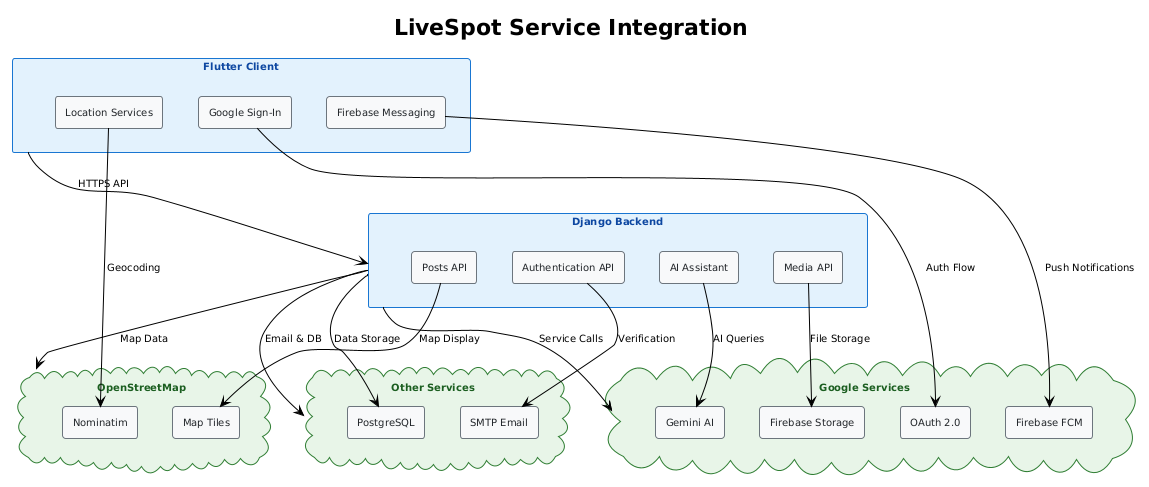
\includegraphics[width=0.7\textwidth]{figures/service_integrations}
    \caption{Service Integration Architecture - Simplified vertical view of external service connections showing the layered integration approach from Flutter client through Django backend to various cloud services}
    \label{fig:service_integrations}
\end{figure}

Figure~\ref{fig:service_integrations} illustrates LiveSpot's streamlined service integration architecture with a clear vertical flow from client to external services. The design emphasizes the strategic layering of services for optimal cost-effectiveness and reliability.

The integration follows a hybrid approach: free services like OpenStreetMap and Nominatim for primary functionality, with Google services providing enhanced features and reliable fallbacks. Firebase services handle real-time capabilities, while traditional infrastructure services like PostgreSQL and SMTP ensure robust data persistence and communication.

%%%%%%%%%%%%%%%%%%%%%%%%%%%%%%%%%%%%%%%%%%%%%%%%%%%%%%%%%%%%%%%%%%%%%%%%%%%%%%%%%%%
\section{Security Architecture}
\label{sec:security_architecture}

\subsection{Authentication and Authorization}

The system implements a JWT-based authentication architecture with hybrid fallback mechanisms, providing secure user access without relying on external authentication providers.

\begin{figure}[h!]
    \centering
    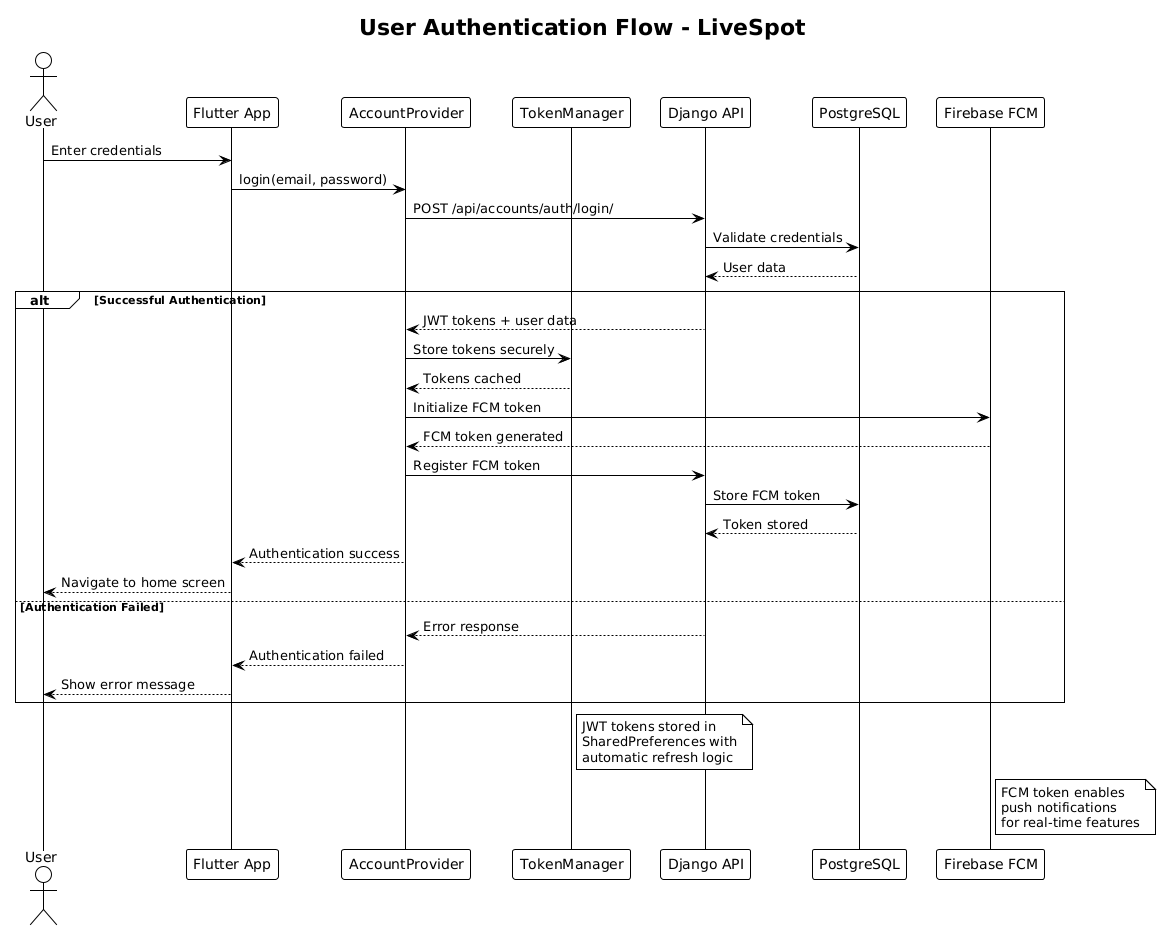
\includegraphics[width=0.95\textwidth]{figures/authentication_sequence}
    \caption{JWT Authentication Sequence Diagram - Complete authentication flow showing JWT token lifecycle, Google OAuth integration, and FCM token registration for secure user access and push notifications}
    \label{fig:auth_flow}
\end{figure}

Figure~\ref{fig:auth_flow} illustrates the comprehensive authentication flow including JWT token generation, Google OAuth integration, and Firebase Cloud Messaging token registration. The sequence demonstrates the secure handshake between Flutter client and Django backend, ensuring authenticated user sessions and push notification capabilities.
\clearpage
\subsection{Security Layers and Protection Mechanisms}

LiveSpot implements a comprehensive multi-layered security architecture that protects user data and system integrity at every level of the application stack.

\begin{figure}[h!]
    \centering
    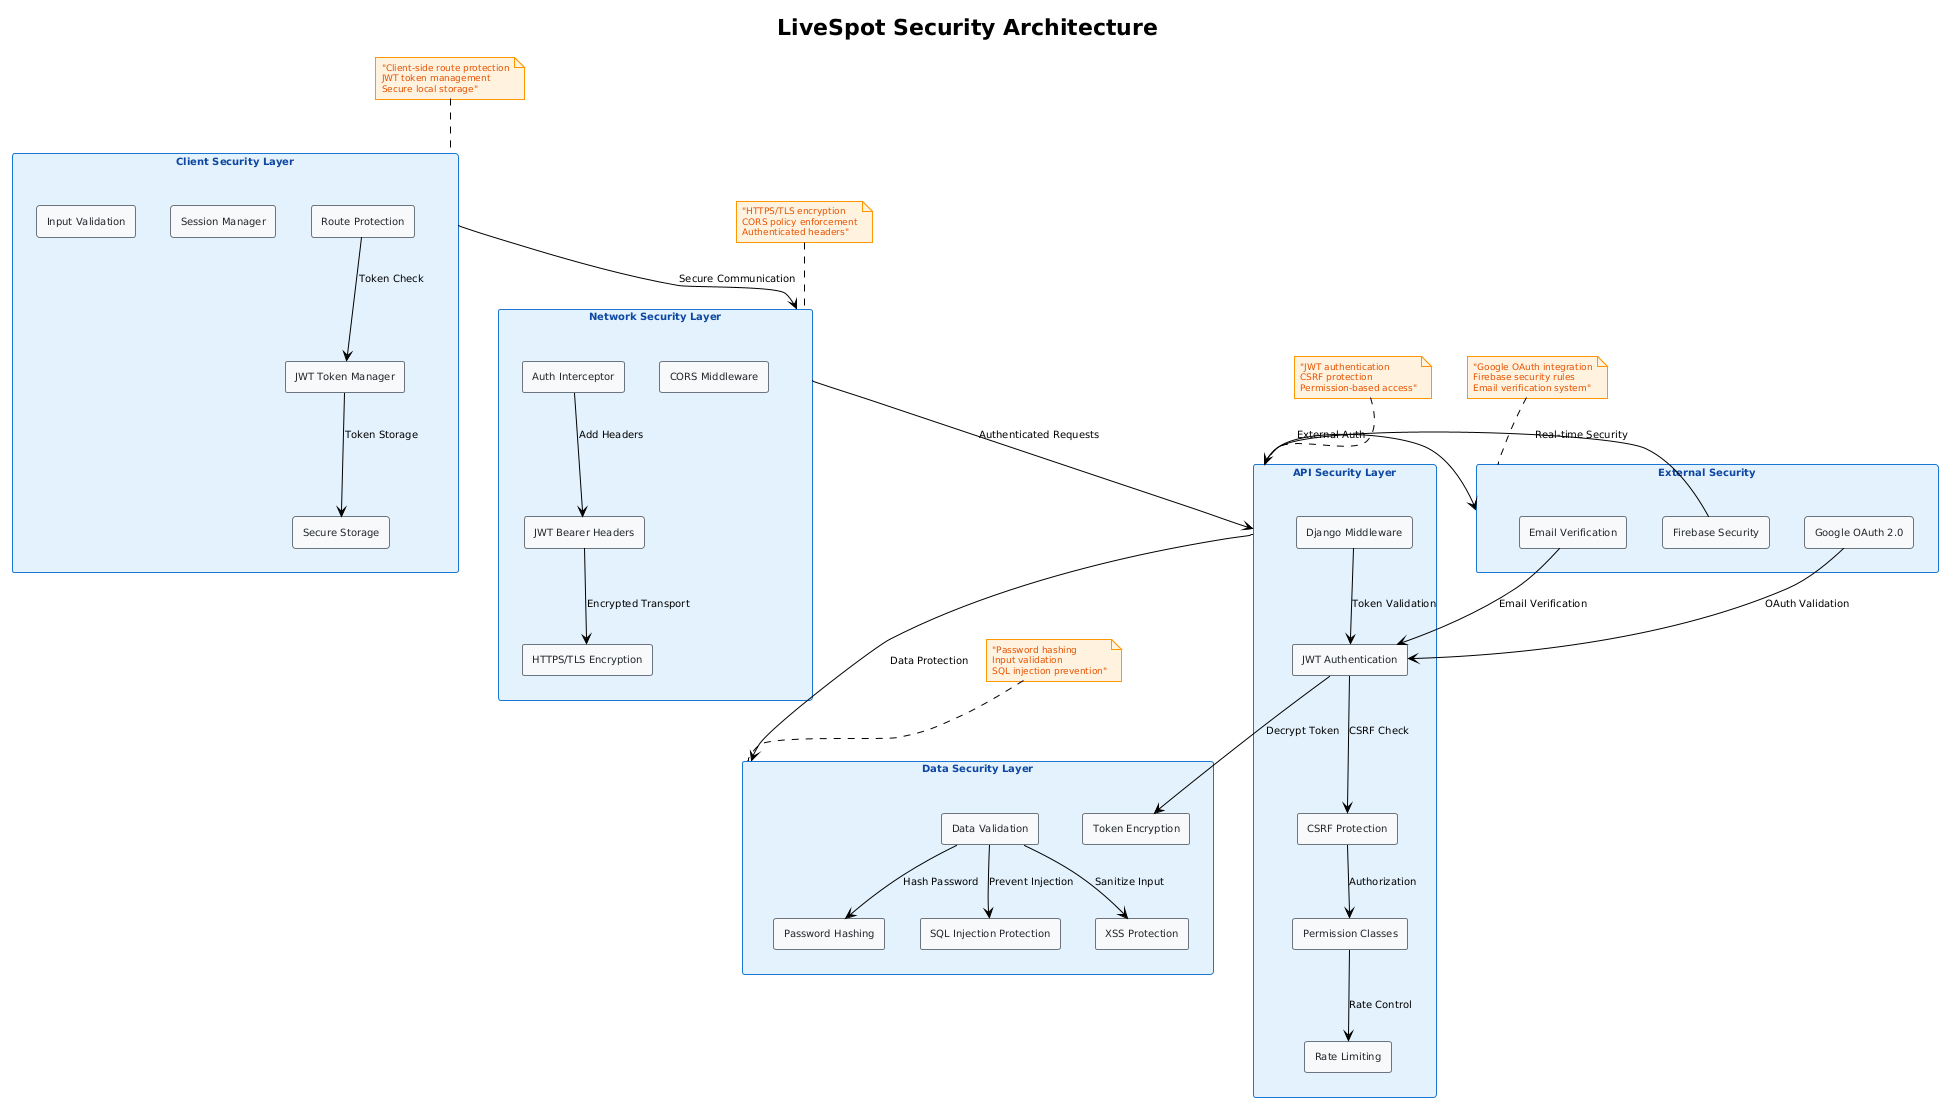
\includegraphics[width=0.8\textwidth]{figures/security_architecture}
    \caption{Security Architecture - Multi-layered security implementation showing client-side protection, network security, API authentication, data encryption, and external service security integration}
    \label{fig:security_architecture}
\end{figure}

Figure~\ref{fig:security_architecture} demonstrates the comprehensive security framework implemented across all system layers. The architecture incorporates client-side route protection, JWT token management with automatic refresh, secure network communications, API-level authentication and authorization, data encryption and validation, and integration with secure external services including Google OAuth and Firebase security features.

%%%%%%%%%%%%%%%%%%%%%%%%%%%%%%%%%%%%%%%%%%%%%%%%%%%%%%%%%%%%%%%%%%%%%%%%%%%%%%%%%%%
\section{Technology Stack}
\label{sec:technology_stack}

\subsection{Frontend Technology Stack}

Rationale for technology selections supporting cross-platform development.

\begin{table}[h!]
    \centering
    \caption{Frontend Technology Stack}
    \label{tab:frontend_stack}
    \begin{tabular}{lll}     
        \toprule
        Category & Technology & Justification \\
        \midrule
        Framework & Flutter & Cross-platform, native performance \\
        State Management & Provider & Simple, efficient state handling \\
        Navigation & Named Routes & Declarative routing system \\
        HTTP Client & Dio & Advanced HTTP features \\
        Local Storage & SharedPreferences & Simple key-value storage \\
        Authentication & Custom JWT & Secure token management \\
        Maps & OpenStreetMap & Free, reliable mapping service \\
        Geocoding & Nominatim + Google & Hybrid geocoding approach \\
        AI Integration & Google Gemini & Advanced conversational AI \\
        \bottomrule
    \end{tabular}
\end{table}
\clearpage
\subsection{Backend Technology Stack}

Server-side technology choices supporting scalability and maintainability.

\begin{table}[h!]
    \centering
    \caption{Backend Technology Stack}
    \label{tab:backend_stack}
    \begin{tabular}{lll}     
        \toprule
        Category & Technology & Justification \\
        \midrule
        Framework & Django REST Framework & Robust API development \\
        Database & PostgreSQL & ACID compliance, performance \\
        Authentication & JWT Tokens & Stateless authentication \\
        Session Management & Custom SessionManager & Session lifecycle control \\
        File Storage & Firebase Storage & Scalable media storage \\
        Push Notifications & Firebase FCM & Reliable message delivery \\
        API Documentation & Django REST Browsable & Interactive API docs \\
        \bottomrule
    \end{tabular}
\end{table}

%%%%%%%%%%%%%%%%%%%%%%%%%%%%%%%%%%%%%%%%%%%%%%%%%%%%%%%%%%%%%%%%%%%%%%%%%%%%%%%%%%%
\section{Summary}

The LiveSpot system design presents a comprehensive, scalable architecture that effectively addresses the requirements for real-time, location-based social networking. The layered architecture with clear separation of concerns enables maintainable code, while the cloud-native approach ensures scalability and reliability. 

The integration of multiple technologies—Flutter for cross-platform development, OpenStreetMap for cost-effective mapping, Firebase for real-time capabilities, Django for robust backend services, and Google Gemini AI for intelligent features—creates a cohesive system capable of supporting large-scale social interactions while maintaining performance and security standards.

The design emphasizes user experience through responsive interfaces, accurate location services, and AI-powered assistance, while maintaining technical excellence through proper architectural patterns, comprehensive security measures, and scalable infrastructure. The detailed architectural diagrams, sequence flows, and component relationships provide a complete blueprint for implementation and future system evolution.

This foundation provides the necessary technical capability to support the application's core mission of creating trustworthy, location-based community reporting and social networking, with built-in scalability to accommodate growth and feature expansion while maintaining cost-effectiveness through the use of open-source and free services where appropriate.
